\documentclass[bachelor,lith,english]{liuthesis}
%% Settings go in settings.tex
\include{settings}
\usepackage{rotating}
\usepackage{color}
\usepackage{pgfplots}
\usepackage{pgfplotstable}
\usepackage{xcolor}
\usepackage{float}
\pgfplotsset{compat=1.18}
\usepackage{fontspec}
\usepackage{subcaption}
\usepackage[normalem]{ulem}
%\newcommand{\revrev}[2]{\textcolor{red}{#2}}
\newcommand{\revrev}[2]{\sout{#1}\textcolor{red}{#2}}
%\newcommand{\revrev}[2]{#2}



% \usepackage{changebar}

\department{Institutionen för datavetenskap}
\departmentenglish{Department of Computer and Information Science}
\departmentshort{IDA}
% If this is a thesis at the cognitive science study programme, use
% the "area" command to generate a proper (?) ISRN
% \area{KOGVET-A}

% Include an external supervisor on the cover page
% \externalsupervisor{Min företagshandledare}
\supervisor{Niklas Carlsson}
\examiner{Marcus Bendtsen}
\titleenglish{Comparing Anomaly Detection Techniques on Offline and Online Log Data}

\titleswedish{Jämförelse av anomaly detection tekniker på offline och online log data}
\thesissubject{Säkra system}

\publicationyear{2025}
\currentyearthesisnumber{14}
\dateofpublication{??}

\author{\parbox{\textwidth}{Carl Arthur\\
Carl Thulin}}

% Two authors
% \author{\parbox{\textwidth}{Ola Leifler\\
%   Alexander Sanner}}

\begin{document}

\chapterstyle{VZ43}

%%% Intro.tex --- 
%% 
%% Filename: Intro.tex
%% Description: 
%% Author: Ola Leifler
%% Maintainer: 
%% Created: Thu Oct 14 12:54:47 2010 (CEST)
%% Version: $Id$
%% Version: 
%% Last-Updated: Thu May 19 14:12:31 2016 (+0200)
%%           By: Ola Leifler
%%     Update #: 5
%% URL: 
%% Keywords: 
%% Compatibility: 
%% 
%%%%%%%%%%%%%%%%%%%%%%%%%%%%%%%%%%%%%%%%%%%%%%%%%%%%%%%%%%%%%%%%%%%%%%
%% 
%%% Commentary: 
%% 
%% 
%% 
%%%%%%%%%%%%%%%%%%%%%%%%%%%%%%%%%%%%%%%%%%%%%%%%%%%%%%%%%%%%%%%%%%%%%%
%% 
%%% Change log:
%% 
%% 
%% RCS $Log$
%%%%%%%%%%%%%%%%%%%%%%%%%%%%%%%%%%%%%%%%%%%%%%%%%%%%%%%%%%%%%%%%%%%%%%
%% 
%%% Code:



\chapter{Introduction}
\label{cha:introduction}
Modern data infrastructures, supercomputer systems and distributed systems generate massive amounts of real-time log data. These logs contain valuable insights into system health, performance, and potential security threats. However, manually analyzing such large and complex datasets is impractical due to their scale. As systems become increasingly interconnected and data volumes grow exponentially, the need for efficient and automated methods to process and analyze log data becomes critical.

Anomaly detection plays a key role in identifying irregular patterns in log data, which may indicate system failures, cyberattacks, or performance degradation. While anomaly detection is widely applied to network traffic analysis, its use in log data remains comparatively underexplored. Using anomaly detection on log data can fill two main purposes, looking back on offline log files to detect previous anomalies, and detecting anomalies on online log data in real-time. Online log data must be processed dynamically, requiring methods that can operate in real-time without relying on complete historical data. In contrast, offline log data can be processed statically, allowing for deeper analysis with access to the entire dataset.

 Machine learning based anomaly detection can enhance anomaly detection specifically on log data, reducing the workload. Also, machine learning in online streaming data enables an automated evaluation of logs, noticing threats before it is to late. This task comes with challenges. As online log data is generated at high speed, the anomaly detector requires to be fast enough to process and analyze data in real-time. Additionally, anomalies are not always obvious, there exist rare anomalies which can go unnoticed when they are compared to normal data. These are difficult for machine learning techniques to detect as they are normally constructed in a generalized way. This paper will analyze different anomaly detection methods within both offline and online log data, comparing the results between the two cases, as well as within each case. 

\section{Motivation}
\label{sec:motivation}
While numerous anomaly detection methods exist and have been widely studied, few studies compare the performance of anomaly detection techniques on both offline and online log data. Existing literature typically focuses on either historical log data or streaming log data, but rarely examines the combination of both. Additionally, the variation in performance for the five algorithms is rarely examined when applied on different types of datasets. Since log data can be utilized for both real-time and past-time anomaly detection, this project aims to evaluate both approaches to gain a deeper understanding of their differences.

\section{Aim}
\label{sec:aim}
In this thesis project, we analyze five anomaly detection techniques on different non-encrypted log datasets. Our objective is to assess and compare their effectiveness in detecting anomalies in different types of data. We focus on two distinct use cases where one involves analyzing historical log data offline, and the other involves processing streamed log data online. 

\section{Research questions}
\label{sec:research-questions}
At a high level, this thesis aims to identify the most effective anomaly detection technique for the given dataset and use case in form of online or offline analysis. To achieve this, five algorithms are tested on two log datasets, allowing for answers to the following questions:

\begin{enumerate}
\item What anomaly detection techniques are the most effective for identifying anomalies offline in different types of non-encrypted log datasets?

\item What anomaly detection techniques are the most effective for identifying anomalies online in different types of non-encrypted log datasets?

\item How does the anomaly detection results on online and offline log data differ, and why? 

\end{enumerate}

The answers to these questions will provide insights into selecting the most suitable anomaly detection techniques for the two use cases, online and offline. Likewise, it will provide information on what algorithm to use for different datasets.

\section{Approach}
\label{sec:approach}
To answer the research questions, this study uses log datasets, which hold suitability for both offline and online streaming data. An iterative approach is applied, refining the methods through multiple attempts to achieve the best results. This study will focus on machine learning-based anomaly detection techniques, evaluating the results of these techniques. The same framework is used for offline and online anomaly detection evaluation. This framework first converts the raw log file into structured logs, then extracts relevant features, which are used for anomaly detection with selected algorithms. For online log data however, this process is done for each log row before handling the next. In contrast, offline learning handles the entire file in each step. The results are evaluated based on recall, precision and F1-score.

\section{Contributions}
\label{sec:contributions}

\begin{itemize}
\item A systematic evaluation of five anomaly detection methods in non-encrypted log datasets to determine their effectiveness for offline and online log data.
\item A comparison and evaluation of how online and offline data impact the results of anomaly detection. We analyze the differences in performance and accuracy, when applying anomaly detection to streaming log data in real-time compared to processing historical log files offline. 
\item Analyzing anomaly detection techniques based on different key values to provide a deeper understanding of the strengths and weaknesses of each technique, allowing informed selection based on the specific use case and purpose.
\end{itemize}

\section{Thesis outline}
To analyze anomaly detection in log data, it is essential to first establish the necessary background, which is provided in Chapter \ref{cha:background}. Section \ref{logdata} introduces log data, followed by an overview of the datasets used in this study in Section \ref{Datasets}. Since the techniques used are based on machine learning, fundamental concepts in this area are covered in Section \ref{ML}, leading to an introduction to anomaly detection in Section \ref{AD}. We then outline earlier work and research on the subject in Section \ref{RelatedWork}. The process of parsing, feature extracting, and anomaly detecting the data is explored in Chapter \ref{cha:method}. The findings are then presented in Chapter \ref{cha:evaluation} and discussed in Chapter \ref{cha:discussion}. Finally, we conclude in Chapter \ref{cha:conclusion}.

%\nocite{scigen}
%We have included Paper \ref{art:scigen}

%%%%%%%%%%%%%%%%%%%%%%%%%%%%%%%%%%%%%%%%%%%%%%%%%%%%%%%%%%%%%%%%%%%%%%
%%% Intro.tex ends here


%%% Local Variables: 
%%% mode: latex
%%% TeX-master: "demothesis"
%%% End: 


\chapter{Background}
\label{cha:background}

\section{Log data}
\label{logdata}
Log datasets consist of several log rows that include automatically generated text about events relevant to a particular system \cite{techtargetlogfile}. In principle, all software applications and systems produce log files. The files contain historical details about the operations, activities, and usage patterns of the system. It provides valuable insights for users, system administrators, or hardware developers, to evaluate the health of the system and determine if it is functioning correctly.

The log files have several different data points included in them such as processes, events and timestamps \cite{techtargetlogfile}. They are also divided into different categories such as system logs, application logs, event logs, and error logs. In this paper, we use system logs and generally recorded events and activities related to the operating system. These logs include details on system modifications, unplanned shutdowns and related messages, hardware malfunctions, errors, resource usage, and various warnings. 

\section{Datasets}
\label{Datasets}
For our research, we utilize Loghub's collection of system logs, which include production data from previous studies as well as logs collected from real systems in a lab environment created for research purposes \cite{zhu2023loghublargecollectionlog}.

\subsection{HDFS-v1}
Hadoop Distributed File System (HDFS) is a distributed system designed to store and manage large-scale data across multiple machines in a fault-tolerant and scalable manner. We will use HDFS-v1 from loghub in our research \cite{zhu2023loghublargecollectionlog}. The logs are sliced into log sequences according to block IDs throughout the work of collecting the data \cite{Wei2010consolelogs}. As shown in Table \ref{tab:dataset}, the HDFS-v1 dataset was collected over a period of $38.7$ hours, contains $11,175,629$ lines, has a total size of $1.47$ GB, and includes manually labeled data through hand-crafted rules to identify anomalies \cite{zhu2023loghublargecollectionlog}. The \revrev{data set}{dataset} will be referred to as HDFS in this paper. 

\subsection{BGL}
BGL is a log dataset from a Bluegene/L supercomputer system at Lawrence Livermore National Labs in Livermore, California. The supercomputer system has $131,072$ processors and $32,768$ GB memory  \cite{zhu2023loghublargecollectionlog}. The logs contain alert and non-alert messages, identified by alert category tags, seen as labels. "-" indicates non-alert messages and any other entry represents an alert message. As shown in table \ref{tab:dataset}, the BGL dataset was collected over a long period of time ($214.7$ days), contains $4,631,261$ lines, has a total size of $719.4$ MB and includes labeled data. 

\begin{table}[t]
    \centering
    \fontspec{Roboto}
    \begin{tabular}{l l c l r r}
        \toprule
        \textbf{Dataset} & \textbf{Description} & \textbf{Labeled} & \textbf{Time Span} & \textbf{\#Lines} & \textbf{Raw Size} \\
        \midrule
        HDFS-v1 & Distributed system & \checkmark & $38.7$ hours & $11,175,629$  & $1.47$ GB  \\
        BGL & Supercomputer system & \checkmark & $214.7$ days   & $4,631,261$ & $719.4$ MB \\
        \bottomrule
    \end{tabular}
    \caption[Dataset details]{Dataset details \cite{zhu2023loghublargecollectionlog}.}
    \label{tab:dataset}
\end{table}

\section{Machine learning}
\label{ML}
In machine learning, statistical learning and optimization methods are used to enable computers to analyze historical data and detect patterns for further assumptions \cite{ucBerkeleyML}. A common assumption in machine learning is that humans train computers to autonomously perform tasks that go beyond basic calculations by learning from their environment through repeated exposure to examples \cite{ElNaqa2015}. Machine learning-based anomaly detection techniques typically operate in three main modes and they are supervised, unsupervised, and semi-supervised learning. The three different modes are figuratively explained in Figure \ref{fig:machine-learning}.

\subsubsection{Supervised learning}
Anomaly detection techniques used in supervised mode require a labeled training set with both anomalous and normal instances \cite{Varun2009Anomaly}. The goal is to create a model capable of predicting whether new data is anomalous or normal. Supervised anomaly detection faces two main challenges, anomalies are much rarer than normal instances in the training data, and accurately labeling data, especially anomalies, is difficult. To address this, some methods introduce artificial anomalies into a normal dataset to create a labeled training set. 

The goal for supervised learning in anomaly detection is to develop a model that maps inputs to outputs, where categorical outputs define a classification task and numerical outputs define a regression task \cite{8406613}. Some examples of tasks for supervised learning is recognition of objects in images \cite{article}, machine translation \cite{10.5555/2969033.2969173}, and filtering spams \cite{788645}.

\subsubsection{Unsupervised learning}
In unsupervised learning, the algorithm is given only input data without any labels, allowing it to train only on an unlabeled dataset \cite{ElNaqa2015}. Unsupervised learning involves solving various problems, such as clustering data points based on a similarity measure \cite{10.1145/331499.331504}, reduce the number of variables and data features with dimensionality reduction \cite{alex2012universityoftoronto}, and model pre-training \cite{10.5555/1756006.1756025}. Clustering is an example that are used for anomaly detection \cite{Varun2009Anomaly}.

\subsubsection{Semi-supervised learning}
Semi-supervised anomaly detection techniques combine elements of both supervised and unsupervised learning methods \cite{ElNaqa2015}. In these techniques, part of the training dataset is labeled while the rest remains unlabeled. As shown in Figure \ref{fig:machine-learning}, semi-supervised learning methods use partially labeled data during training. The more labeled data you require in the training set, the greater the need for human-machine interaction. 

\begin{figure}[t]
    \centering
    
\includegraphics[width=0.9\linewidth]{figures/learningmethods.pdf}
    \caption[The different modes of machine learning]{The different modes of machine learning. Created in BioRender \cite{biorendermodesofmachinelearning}}.
    \label{fig:machine-learning}
\end{figure}

\section{Anomaly detection}
\label{AD}
Anomaly detection is about finding patterns in data that is not in line with the expected behavior, these abnormal patterns are referred to as anomalies or outliers \cite{Varun2009Anomaly}. Anomalies are patterns in data that does not comply with the defined normal behavior, illustrated in Figure \ref{fig:anomalies} where $O_1$, $O_2$ and $O_3$ are anomalies, being far away from the normal regions $N_1$ and $N_2$ (considered normal as most observations lie there). The usage field of anomaly detection is wide, spanning from fraud detection in credit cards to military surveillance. Within this span lies intrusion detection for cybersecurity, which is the usage area of this project.

Defining what is normal and abnormal data is not an easy task, nor is it easy to define an anomaly. Varun et al. \cite{Varun2009Anomaly} classifies anomalies into following three categories.

\subsubsection{Point Anomalies} If a single data instance stands out as anomalous compared to the rest of the dataset, it is referred to as a point anomaly. This is the most basic type of anomaly, and the easiest to detect as it deviates from the rest of the data.

\subsubsection{Contextual Anomalies} A data instance is considered a contextual anomaly if it is anomalous within a specific context but does not have to appear as an anomaly in other circumstances.

\subsubsection{Collective Anomalies} When a group of related data instances deviates from the the overall dataset, that group is considered a collective anomaly. However, this does not necessarily mean that all instances are anomalies on their own, but their combined occurrence forms an anomaly. 

\begin{figure}[t]
    \centering
    
\includegraphics[width=0.75\linewidth]{figures/anomalies.pdf}
    \caption[Simplified example of anomalies]{Simplified example of anomalies. Created in BioRender \cite{biorenderanomalies}.}
    \label{fig:anomalies}
\end{figure}


\subsection{Offline anomaly detection methods} 
An offline anomaly detection technique refers to the process of analyzing previously collected data, not in real time, to identify anomalies. This approach processes the entire dataset at once, instead of continuously monitoring incoming data, and is typically used for analyzing historical data or if real-time detection is not required.

\subsubsection{Isolation Forest}
Isolation Forest (IF) is an unsupervised machine learning method used for anomaly detection. It is a decision-tree-based algorithm using isolation trees \cite{CortesIF}. It's functionality is based on randomly splitting data along feature values, and isolating rare observations in fewer splits. Since anomalies differ from the majority of data, they should be easier to detect. Isolation trees recursively separates data until each point is isolated, while common points require more separations, anomalies require few and are quickly isolated \cite{Fei2008IsolationForest}. The depth of the tree then gives a measure of how anonymous the point is, a higher depth gives less indication of anomaly, while lower depth indicates anomaly. To put this in perspective, using 1000 trees, anomalies has an average path (number of edges traversed) of $4.02$ and normal points has an average path of 12.82 \cite{Fei2008IsolationForest}. Using IF in anomaly detection is a two stage process, firstly there is a training stage, then a evaluating stage. 

In the \textbf{training stage} isolation trees are built recursively dividing the training data until all instances are isolated, or a certain tree height is reached (resulting in an incomplete model). The tree height \( \ell \) is determined based on the sub-sampling size \( \psi \) using the formula 
\begin{equation*}
l = \lceil \log_2(\psi) \rceil
\end{equation*} 
and indicates the average height. Since no \revrev{anomaly's}{anomalies} should reach a height higher than average, only data points with shorter than average path are of interest. 

IF has two input parameters, sub-sampling size \( \psi \) and number of trees \textit{t}. The sub-sampling size \( \psi \) controls the training data size, however when it's increased to a desired value there is no need to increase further, as it leads to higher processing time and increased memory size. The recommended value is \( \psi = 256 \) \cite{Fei2008IsolationForest}. The number of trees \textit{t} controls the ensamble size. The default value is  \( \textit{t} = 100 \), higher value normally does not increase accuracy. 

The \textbf{evaluating stage} derives an anomaly score \textit{s} based on an expected path length, calculations for this can be found in Fei Tony et al paper \cite{Fei2008IsolationForest}. The anomaly score \textit{s} holds a value $0 < s \leq 1$. If  \textit{s} is very close to 1, it's definitely an anomaly. If  \textit{s}  is much smaller than $0.5$, they are safe to be regarded as normal instances. Lastly, if all instances return $s\approx 0.5$ the whole set is considered not having any distinct anomaly. 

\subsubsection{LogClustering}
LogClustering is an unsupervised anomaly detection technique that groups logs into clusters, making it easier to identify log-based issues \cite{7883294}. It also leverages a knowledge base to determine whether specific log sequences have occurred before. There are two different phases of the LogClustering operations, construction phase and production phase. During the construction phase, the vectorized log sequences are clustered and a representative sequence from each cluster is stored in a knowledge base. In the production phase, logs are processed the same way, and new sequences are checked against the knowledge base. Finally, the knowledge base is updated with the new clusters. 

Figure \ref{fig:LogClustering_image} illustrates the three main steps of the process \cite{7883294}. The first step is log clustering, where the similarity between log sequences is calculated using the agglomerative hierarchical clustering technique, allowing them to be grouped into clusters. In the second step, extracting representative log sequences, the centroid of each cluster is selected as its representative log sequence. Finally, in the checking recurrence step, each representative log sequence is examined to determine whether it has previously appeared in the knowledge base. 

\begin{figure}[t]
    \centering
    
\includegraphics[width=0.9\textwidth]{figures/Logclustering-2.pdf} 
    \caption[Illustration of the key stages in the LogClustering algorithm]{Illustration of the key stages in the LogClustering algorithm. Created in BioRender \cite{biorenderlogclustering}.}
    \label{fig:LogClustering_image}
\end{figure}

\subsubsection{PCA}

Principal Component Analysis (PCA) is an unsupervised statistical machine learning technique widely used for anomaly detection and dimension reduction \cite{Shilin2017experiencereport}. That is, reduce the amount of variables but still preserve the valuable information. In fact, it is perhaps the best-known statistical method to achieve data separation for anomaly detection\cite{Kun2018On-LineAnomalydetection}. The core idea is to transition high dimensional data onto a new coordinate system defined by \textit{k} principal components, where \textit{k} is smaller than the original data's dimension. PCA calculates \textit{k} by  determining axes that account for the largest amount of variance in the data\cite{Shilin2017experiencereport}. 

Once the principal components are found, they are ranked based on the contribution to the total variance, where lower-dimensional \textit{k} represent the core behavior and higher dimensional represent less relevant or noisy information. By doing so, the data is transformed into a lower-dimensional space, while still preserving essential characteristics. The new coordinate system can now be used in different ways, for instance in anomaly detection. To deviate normal data from anomalies, the principal components are split into two groups. Data that aligns with the lower-dimensional subspace is considered normal, while data associated with the higher-dimensional subspace is classified as anomalous \cite{Kun2018On-LineAnomalydetection}.

\revrev{}{\subsubsection{Support Vector Machines}Support Vector Machines (SVM) is an supervised machine learning algorithm used for classification and regression tasks. It was originally designed to distinguish between two distinct data classes. When presented with such data, the algorithm identifies an optimal linear decision boundary known as a hyperplane that separates the classes while maximizing the margin between them. The margin refers to the largest possible distance the boundary can maintain from the closest data points on either side without misclassifying them. These closest data points, which the margin touches, are known as "support vectors" and are critical in defining the position and orientation of the hyperplane \cite{Mahadevan2009Fault}. 
}

\subsection{Online anomaly detection methods}
 Online anomaly detection refers to the process of identifying unusual patterns or deviations in real-time data. Online detection must process incoming data dynamically, making decisions without access to the entire historical dataset or future logs. This creates needs for efficient algorithms that can handle streaming data, adapt to new patterns and detect anomalies. 

\subsubsection{One-Class SVM}
\revrev{Support Vector Machines (SVM) were initially designed to distinguish between two distinct data classes. When presented with such data, the algorithm identifies an optimal linear decision boundary known as a hyperplane that separates the classes while maximizing the margin between them. The margin refers to the largest possible distance the boundary can maintain from the closest data points on either side without misclassifying them. These closest data points, which the margin touches, are known as "support vectors" and are critical in defining the position and orientation of the hyperplane \cite{Mahadevan2009Fault}. }{}


The One-Class SVM technique is a variant of the original support vector machine algorithm first proposed by Schölkopf et al. \cite{Schölkopf2001Estimating}, which is more specifically presented for outlier detection. The goal is to separate the outlier samples from normal samples. The One-Class SVM however only needs the normal data points while training, in contrast to SVM which needs both. One-Class SVM learns a boundary based on the majority of training data that represents normal system behavior. When a new test sample is evaluated, it is considered normal if it lies within this learned boundary, otherwise it is flagged as an anomaly. To handle more complex, non-linear patterns in the data, a kernel function is applied, which transforms the input data into a higher-dimensional space where a linear separation becomes possible \cite{Mahadevan2009Fault}. Figure \ref{fig:oneclassSVM_image} illustrates the basics of the One-Class SVM. Here, the green instances represents normal data points, red represents anomalies, and "d" represents the distance to the boundary, anything within the boundary is considered anomalous, and outside is considered normal. 



\begin{figure}[t]
    \centering
    \includegraphics[width=0.7\textwidth]{figures/OneclassSVM.pdf} 
    \caption[Graphical illustration of One-Class SVM]{Graphical illustration of One-Class SVM. Created in BioRender \cite{biorenderoneclasssvm}.}
    \label{fig:oneclassSVM_image}
\end{figure}


\subsubsection{Half-Space Trees}
\label{HST}
Half-Space Trees (HST) are an online version of Isolation Forest (IF) \cite{riverWebsite}. The anomaly detection technique performs well for training on both normal data and data with anomalies, particularly effective for datasets with few anomalous data points \cite{SweeChuan2011FastAnomalyDetectionForStreamingData}. Unlike the IF method, which requires static data and does not update continuously \cite{Fei2008IsolationForest}, HST is an online anomaly detection technique that adapts to new data points without requiring model reconstruction~\cite{SweeChuan2011FastAnomalyDetectionForStreamingData}.

The HST method is a tree-based algorithm where each tree consists of nodes that capture the mass (number of data items) within a specific region of the data stream \cite{SweeChuan2011FastAnomalyDetectionForStreamingData}. Lower mass values indicate anomalies, while higher mass values suggest normal data. The data stream is divided into two types of windows, the reference and the latest windows. The reference window is used to learn the mass value, which eventually determines whether the data in the latest window is anomalous. When the latest window is full, the mass value is updated with new data, and the reference window is updated accordingly. The content of the latest window is then erased and is ready to receive new data. This process continues until the data stream ends.

\section{Related work}
\label{RelatedWork}
\subsubsection{Log data}
Log data is an area in which there has been much research prior to our study and there exist many different log \revrev{data sets}{datasets} from different machines. There have been several evaluations of HDFS datasets \cite{Shilin2017experiencereport} \cite{ZEUFACK2021100030Anunsupervisedanomalydetection} \cite{zhu2023loghublargecollectionlog} \cite{Wei2010consolelogs} \cite{Pinja2017Drain} \cite{Guo2021LogBERT} \cite{Le2022LogBased} and BGL datasets \cite{Guo2021LogBERT} \cite{Le2022LogBased} \cite{Shilin2017experiencereport}\cite{zhu2023loghublargecollectionlog}\cite{Pinja2017Drain}, these two datasets are also used in our research. To utilize log data effectively, log parsing is required \cite{zhu2019toolsbenchmarksautomatedlog}. Therefore, we use Drain, which outperforms existing online log parsers in both accuracy and efficiency, as well as surpassing state-of-the-art offline parsers\cite{Pinja2017Drain}, which is also research on by Zhu et al \cite{zhu2019toolsbenchmarksautomatedlog}. To enable the use of anomaly detection techniques, feature extraction is necessary. The subject has been extensively studied in prior research \cite{Shilin2017experiencereport} \cite{Gautam2018bigdatarealtime} and highlights the two grouping techniques that we will use, sliding and session window.

\subsubsection{Online data}
There has been previous research within the area of anomaly detection on streaming data, that is, real-time data \cite{Hasani2017robustanomaly}\cite{ZEUFACK2021100030Anunsupervisedanomalydetection}. Hasani \cite{Hasani2017robustanomaly} discusses the importance of detecting anomalies in real-time, to instantly alarm on threats before they are stored. He highlights the importance of algorithms needing a low processing time, eventually at the cost of accuracy. Additionally a comparison is done of nine fast anomaly detection techniques performed on timeseries-stamped log-datasets, evaluating the number of anomalies found. However, only investigating these algorithms creates a research gap for other anomaly detection techniques such as Half-Space Trees and One-Class SVM. 

Zeufack et al. \cite{ZEUFACK2021100030Anunsupervisedanomalydetection} studies unsupervised anomaly detection on streaming log files, and proposes a new real-time method that can process log messages as they are generated, without studying the log-file beforehand. However they only use one anomaly detection method and no comparison is done between others. This research highlights the need of evaluating techniques based on their ability to detect anomalies, while leaving room for more research to be done in the area and analyzing other techniques on online log data.  

\subsubsection{Offline data}
The area of anomaly detection on offline data has previously been studied. Munir et al. \cite{Munir2019Comparativeanalysis} looks into anomaly detection on data comparing deep learning-based anomaly detection methods with traditional methods. They do this by evaluating the results on precision, area under ROC curve, area under precision-recall and inference time. However, the datasets used in the study are not log-based and they base their results on different metrics than this report. 

\subsubsection{Anomaly Detection}
Anomaly detection has a wide range of usage areas, and previous research has been conducted to evaluate their results, identify use areas, and outline relevant techniques \cite{Callegari2017anoverviewofselectedmethods}\cite{Varun2009Anomaly}. Anomaly detection techniques have been widely explored in previous research, with machine learning-based approaches being the most commonly used \cite{Shilin2017experiencereport} \cite{Wei2010consolelogs} \cite{ZEUFACK2021100030Anunsupervisedanomalydetection}. Various methods have been applied to detect anomalies in datasets, including PCA \cite{Shilin2017experiencereport}\cite{Munir2019Comparativeanalysis}\cite{Mahadevan2009Fault},
Isolation Forest \cite{Munir2019Comparativeanalysis}\cite{Awad2023anomalydetectionandsecurityenhancement}\cite{Lukito2023Comparison},
LogClustering \cite{7883294}, Half-Space Trees \cite{SweeChuan2011FastAnomalyDetectionForStreamingData}, and One-Class SVM \cite{Lukito2023Comparison}\cite{Mahadevan2009Fault}. However, they have not been compared against each other on log-data. 
\chapter{Method}
\label{cha:method}
In this chapter, a step by step description of the process of detecting anomalies in a raw unstructured log file is provided. 
\section{Framework}
To perform anomaly detection on log data, the data has to be transformed and prepared to fit the selected anomaly detection techniques. The used method of choice consists of four steps: 

\begin{enumerate}
    \item \textbf{Log collection}: Has already been completed and is provided in the selected datasets, this study focuses on the remaining steps.
    \item \textbf{Log parsing}: Structures the log files.
    \item \textbf{Feature extraction}: Creates numerical vectors based on the structured data.
    \item \textbf{Anomaly detection}: Uses the vectors created as input for the algorithms to detect anomalies.
\end{enumerate}
An overview of this process is shown in Figure \ref{fig:method-process}.

For the offline log data evaluations, the entire log file will be handled at once. That is, the entire log file will first be parsed and structured, followed by feature extraction and finally, anomaly detection will be performed on the entire dataset at once. In contrast, for the online log data evaluation, the entire log file will still be parsed at once, as parsing each row individually does not impact the results. However, feature extraction will be performed dynamically, processing one structured log row at a time. Each extracted feature vector will be immediately analyzed for anomalies before moving on to the next log row. 


\begin{figure}[t]
    \centering
    
\includegraphics[width=1\linewidth]{figures/Method.pdf}
    \caption[Methodology overview of our framework]{Methodology overview of our framework. Created in BioRender \cite{biorendermethodology}.}
    \label{fig:method-process}
\end{figure}


\section{Log parsing}
Logs are generated by various systems and often contain valuable information about the system. However, these logs are stored in raw text formats, making it difficult to process. The huge volume logs combined with the unstructured representation makes it impractical to manually inspect \cite{zhu2019toolsbenchmarksautomatedlog}.  Log parsing is therefore essential to prepare the data in a structured way for the anomaly detection algorithms, making it the first step in log data analysis. By extracting the key attributes, going from free text raw-log messages to structured form, log parsing enables the possibility to use automated anomaly detection techniques to detect patterns on log data.

The log messages are generated by a logging statement in the source code, and consists of a message header and message content. The logging framework has determined the header and is rather easy to extract (e.g. of headers are timestamps and level). It is however harder to structure the free-text message content, because it's a formation of constant strings and variable values \cite{zhu2019toolsbenchmarksautomatedlog}. The goal of log parsing is to transform these messages into structured event templates by identifying the core event type while filtering out dynamic variables. This abstraction enables more efficient log analysis and anomaly detection.

A presentation, analyses and evaluation is performed by Zhu et al \cite{zhu2019toolsbenchmarksautomatedlog} on $13$ different log parsers on $16$ datasets. They go through each algorithm, evaluating based on accuracy, robustness and efficiency. The top performing algorithm was shown to be Drain, providing the highest accuracy on average, but shows smallest variance combined with robustness when changing volumes of logs. Pinja et al \cite{Pinja2017Drain} also performed an analysis, evaluating Drain on five real world log data sets. The results show that Drain demonstrate the highest accuracy on four of the sets, and a comparable accuracy on the fifth while also improving running time by $51.8$\textasciitilde $81.47$\%.  Additionally, most log parsing methods focus only on offline batch processing. However, Drain is a method suitable for both online and offline log parsing \cite{Pinja2017Drain}. Therefore, Drain is the method selected for the HDFS data. Due to time limitations, we used an already parsed BGL dataset \cite{4273008} \cite{zhu2023loghublargecollectionlog}.

\subsection{Drain}
Drain is a method supporting both online and offline log parsing that only requires the raw log messages \cite{Pinja2017Drain}. Drain can automatically extract log messages, split it into log groups using a parse tree with fixed depth, (i.e. all leaf nodes are found at the same depth). This is done by preprocessing the log message by regular expressions. Then searching for a log group (leaf nodes) by following the rules of the internal nodes of the tree. When a suitable group is found, the message is matched with that log event, else a new log group is created. By using a parse tree with fixed depth, the technique avoids comparing log messages to every log group, saving time and efficiency. The log group contains a log event and \revrev{an}{a} log ID, the first describes the log message of the group (the message content described above). The second, log ID, records the ID of log messages in that group. In this project, an existing implementation by the LogPai team was used.


\section{Feature extraction}
Once the parsed log messages are created, the structured log messages need to be converted into numerical features for machine learning algorithms to be able to process them. Therefore, a feature extraction is needed to encode the parsed log messages further. This can be done using grouping techniques, such as fixed window, sliding windows and session windows. By doing so, feature vectors are created representing the number of occurrences for a specific event. All feature vectors can together form a feature matrix \cite{Shilin2017experiencereport}. 

\subsection{Fixed Window}
\label{fixedWindowSection}
Fixed window is a timestamped based method. The logs are divided into windows based on the fixed time duration, where the window size $\Delta t$ is a constant value \cite{Shilin2017experiencereport}. Therefore, the number of windows depend on the predefined window size, and the windows do not overlap with each other's time boundaries \cite{Gautam2018bigdatarealtime}. Further, logs that occur in the same windows are called a log sequence. A demonstration of fixed window is provided in Figure \ref{fig:Fixed-window}.

\begin{figure}[t]
    \centering
    \includegraphics[width=1\linewidth]{figures/Fixed_window.pdf}
    \caption[Fixed window approach]{Fixed window approach, where the \textcolor{orange}{orange} and \textcolor{blue}{blue} circles represent different types of event. Created in BioRender \cite{biorenderfixedwindow}.}
    \label{fig:Fixed-window}
\end{figure}



\subsection{Sliding Window}
Unlike fixed windows, sliding windows are defined by two key parameters, window size and step size, where the windows overlap if the window size is greater than step size \cite{Gautam2018bigdatarealtime}. In Figure \ref{fig:sliding-window} it is shown that the logs that occur in the same sliding window are grouped as a log sequence. Logs may also be duplicated in several sliding windows due to the overlap that occurs \cite{Shilin2017experiencereport}. 

\begin{figure}[t]
    \centering
    
\includegraphics[width=1\linewidth]{figures/Slidingwindow.pdf}
    \caption[Sliding window approach]{Sliding window approach, where the \textcolor{orange}{orange} and \textcolor{blue}{blue} circles represent different types of event. Created in BioRender \cite{biorenderslidingwindow}.}
    \label{fig:sliding-window}
\end{figure}

\subsection{Session Window}
The session window approach is however based on identifiers rather than timestamps. These identifiers help to differentiate execution paths in log datasets \cite{Shilin2017experiencereport}. For example, the HDFS logs use \textit{block\_id} to track operations as allocation, writing, replication or deletion of blocks. By leveraging these identifiers the logs can be grouped into session windows, where each session window is associated with an identifier. This is demonstrated in Figure \ref{fig:session-win}, where the number of event types are grouped \revrev{in}{by} sessions. 

\begin{figure}[t]
    \centering
    
\includegraphics[width=1\linewidth]{figures/Session window.pdf}
    \caption[Session window approach]{Session window approach, where the \textcolor{orange}{orange} and \textcolor{blue}{blue} circles represent different types of event occurring in one session. Created in BioRender \cite{biorendersessionwindow}.}
    \label{fig:session-win}
\end{figure}

\section{Anomaly detection}
Once the vector matrix is constructed, the process of detecting anomalies can begin. This study employs machine learning-based approaches, specifically leveraging \textbf{PCA}, \textbf{LogClustering}, \textbf{Isolation Forest}, \textbf{Half-Space Trees} and \textbf{One-Class SVM} as the selected algorithms. A detailed description of these methods is provided in Section \ref{AD}. These are all unsupervised machine learning-based methods (described in Section \ref{ML}), as they align most closely with real-world scenarios where labeled data is unavailable.  \revrev{}{Additionally, \textbf{SVM} was implemented using supervised training, this result serves as a benchmark for the unsupervised methods. This allows an estimation of an upper bound of achievable performance when labels are 
available, and compare how well unsupervised methods perform. }

\revrev{}{The methods were selected to represent different categories of anomaly detection approaches, such as tree-based, clustering based, and statistical techniques. This was done to ensure a broad perspective in our evaluation. Additionally, the chosen algorithms have demonstrated promising results in previous research, which further motivated their inclusion in this study.} 
For PCA, Isolation Forest and LogClustering, open source implementations by the LogPai team were used \cite{Shilin2017experiencereport}.  We implemented the Half-Space Trees and One-Class SVM algorithms using the River library in Python \cite{montiel2021river}, where a stochastic implementation of the One-Class SVM algorithm has been created to handle online scenarios.



\section{Implementation}
In our experiments, we used $80$\% of the dataset as a training set and remaining $20$\% as a test set for the online data. This provides enough data for both training and testing, while correlating with a real world scenario. \revrev{}{ Additionally, the online methods trained on normal data exclusively.} For the offline data however, the entire file was used as training, this also correlates with a real world situation where one would have access to the entire file. The HDFS dataset was first log parsed using Drain, then feature extracted with session windows based on \textit{block\_id} before implementing the different anomaly detectors. The online implementations on the HDFS dataset were initially trained in an offline setting, as access to the entire training data reflects a real-world scenario. The testing was then implemented in an online environment. For the BGL dataset, because of time limitations an already log parsed file in a structured format was used \cite{zhu2023loghublargecollectionlog} \cite{4273008}\revrev{}{, since log parsing with Drain would provide the same results}. Since there is no feature in the BGL dataset that can be used to create session windows, sliding windows was used as a feature extraction method, since it performs better on BGL than fixed window \cite{Shilin2017experiencereport}. The offline sliding window size was timestamp-based while the online sliding window size was based on the number of log-rows, to simplify computation. Both BGL implementation scenarios were implemented with an event count vector. Lastly, for One-Class SVM a standard scaler was used after the feature extraction to preprocess the data for better results \cite{montiel2021river}. For Half-Space Trees, a MinMaxScaler was applied for the same purpose. \revrev{}{The LogClustering algorithm was trained only on normal data, unlike the other two offline algorithms which used both normal and anomalous data in the training phase. While SVM trained in a supervised setting, with a labeled dataset to serve as a benchmark.} The code was written in Python 3.11.6 on a macOS system running on a MacBook Air with an Apple M2 chip ($8$-core CPU, $8$-core GPU) and $16$ GB unified memory. 
%%% lorem.tex --- 
%% 
%% Filename: lorem.tex
%% Description: 
%% Author: Ola Leifler
%% Maintainer: 
%% Created: Wed Nov 10 09:59:23 2010 (CET)
%% Version: $Id$
%% Version: 
%% Last-Updated: Wed Nov 10 09:59:47 2010 (CET)
%%           By: Ola Leifler
%%     Update #: 2
%% URL: 
%% Keywords: 
%% Compatibility: 
%% 
%%%%%%%%%%%%%%%%%%%%%%%%%%%%%%%%%%%%%%%%%%%%%%%%%%%%%%%%%%%%%%%%%%%%%%
%% 
%%% Commentary: 
%% 
%% 
%% 
%%%%%%%%%%%%%%%%%%%%%%%%%%%%%%%%%%%%%%%%%%%%%%%%%%%%%%%%%%%%%%%%%%%%%%
%% 
%%% Change log:
%% 
%% 
%% RCS $Log$
%%%%%%%%%%%%%%%%%%%%%%%%%%%%%%%%%%%%%%%%%%%%%%%%%%%%%%%%%%%%%%%%%%%%%%
%% 
%%% Code:






\chapter{Evaluation}
\label{cha:evaluation}

\section{Evaluation method}

The results of our anomaly detection techniques are first classified as True Positives (TP), True Negatives (TN), False Positives (FP) and False Negatives (FN) as shown in Table \ref{tab:anomaly_matrix}. With these classified data, we evaluate the techniques based on their precision:
$$ 
\text{Precision} = \frac{\text{TP}}{\text{TP} + \text{FP}} \quad \text{,}
$$
which captures how many of the predicted anomalies are actually true anomalies. A high precision means that fewer of the normal instances are incorrectly predicted as anomalies, and therefore reducing the FP rate. It is especially important in cases where FP wastes to much time and resources. With high precision, we ensure that the anomalies predicted by the anomaly detection technique are more likely to be real anomalies. To further understand the model's performance, we also evaluate the detection techniques based on their recall: 
$$
\text{Recall} = \frac{\text{TP}}{\text{TP} + \text{FN}} \quad \text{,}
$$
to evaluate how many true anomalies the model identifies. A high recall would mean that fewer actual anomalies are missed, which helps reduce the number of FN. If not missing an anomaly is of crucial importance, a high recall is very important to ensure that all potential issues are captured. Often, prioritizing recall and finding as many anomalies as possible comes at the cost of increasing FP. Finally, we also want to investigate the relationship between precision and recall. To evaluate this, we use \revrev{F1 score}{F1-score}, calculated as: 
$$
\text{F1-score} = 2 \times \frac{\text{Precision} \times \text{Recall}}{\text{Precision} + \text{Recall}} \quad \text{,}
$$
this metric is designed to balance the mean of precision and recall, and provides a single value that reflects the model's overall performance by balancing both precision and recall. The value gives us a good understanding of which technique is best when precision and recall are equally important. 

\begin{table}[t]
\centering
\fontspec{Roboto}
\begin{tabular}{|c|c|c|}
\hline
 & \textbf{Predicted Anomaly} & \textbf{Predicted Normal} \\
\hline
\textbf{Actual Anomaly} & True Positives (TP) & False Negatives (FN) \\
\hline
\textbf{Actual Normal} & False Positives (FP) & True Negatives (TN) \\
\hline
\end{tabular}
\caption{Matrix of Anomalies.}
\label{tab:anomaly_matrix}
\end{table}

\section{Results}
In this section the experimental results are provided. First, the results on each dataset are presented where all five algorithms are applied for both datasets. Then, results for offline and online anomaly detection are displayed. In all tests, the goal is to achieve the highest possible F1-score.

\subsection{HDFS} 
The results of the anomaly detectors when applied on the HDFS dataset are shown in Figure~\ref{fig:hdfs-v1-results}. The results shown are precision, recall and F1- score for \revrev{}{SVM}, Isolation Forest, PCA, LogClustering, Half-Space Trees and One-Class SVM. \revrev{}{SVM, serving as a benchmark for the other algorithms, demonstrates high results.} LogClustering showed the best results \revrev{}{out of the unsupervised methods }in all three evaluation metrics. PCA also demonstrates good results, providing the second best results in all three evaluation parameters. Isolation Forest exhibits relative consistent performance, with precision, recall, and F1-score values remaining closely aligned. Half-Space Trees provides a high precision, but a low recall resulting at an F1-score of $33$\%. One-Class SVM shows the weakest results out of all algorithms, however the results are fairly stable. For each algorithm, precision yields the highest score, whereas recall consistently results in the lowest.

\begin{figure}[t]
    \centering
    {\fontspec{Roboto}
    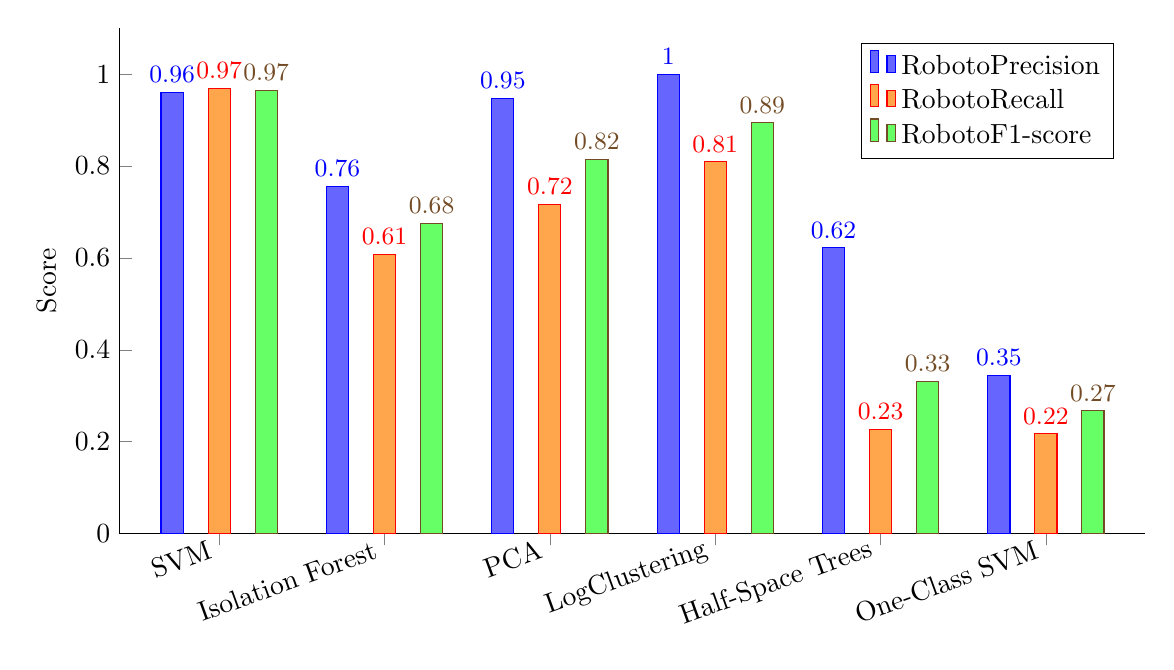
\begin{tikzpicture}
        \begin{axis}[
            ybar,
            bar width=8pt,
            x=2.1cm,
            width=14cm,
            height=8cm,
            enlarge x limits=0.12,
            ylabel={Score},
            symbolic x coords={SVM, Isolation Forest, PCA, LogClustering, Half-Space Trees, One-Class SVM},
            xtick=data,
            xticklabel style={rotate=20, anchor=east},
            legend style={at={(0.97,0.97)}, anchor=north east, font = \fontspec{Roboto}},
            legend cell align=left,
            ymin=0, ymax=1.1,
            nodes near coords,
            nodes near coords align={vertical},
            every node near coord/.append style={font=\small},
            ylabel near ticks,
            axis x line*=bottom,
            axis y line*=left
        ]
        %Precision
        \addplot+[style={fill=blue!60}, bar shift=-17pt] coordinates {
           (SVM, 0.961)
            (Isolation Forest, 0.756)
            (PCA, 0.947)
            (LogClustering, 1.000)
            (Half-Space Trees, 0.622)
            (One-Class SVM, 0.345)
        };
        %Recall
        \addplot+[style={fill=orange!70}, bar shift=0pt] coordinates {
            (SVM, 0.969)
            (Isolation Forest, 0.608)
            (PCA, 0.716)
            (LogClustering, 0.809)
            (Half-Space Trees, 0.227)
            (One-Class SVM, 0.217)
        };
        %F1
        \addplot+[style={fill=green!60}, bar shift=17pt] coordinates {
        (SVM, 0.965)
            (Isolation Forest, 0.675)
            (PCA, 0.815)
            (LogClustering, 0.894)
            (Half-Space Trees, 0.332)
            (One-Class SVM, 0.267)
        };
        \legend{Precision, Recall, F1-score}
        \end{axis}
    \end{tikzpicture}
    }
    \caption[Comparison of anomaly detection techniques on HDFS dataset]{Comparison of anomaly detection techniques on HDFS dataset \revrev{}{(results rounded to two decimal places)}.}
    \label{fig:hdfs-v1-results}
\end{figure}

\subsection{BGL}

This section provides the results of each algorithm evaluated on the BGL dataset. Since a sliding window approach was applied, different window sizes and step sizes were explored. The corresponding results for these are also shown. The evaluated window sizes are 4, 6, and 8 hours, each paired with step sizes of 1, 2, and 3 hours, respectively.

\revrev{}{\subsubsection{SVM}
The results shown in Figure \ref{fig:svm_all_metrics} indicate very similar performance across the different window and step sizes. Precision remains consistently at 100\%, while recall varies more. The highest recall is achieved with a window size of 8 and a step size of 3. This slightly higher recall results in the best F1-score, reaching 99.8\%.
}

\begin{figure}[t]
    \centering
    % Shared legend at the very top, centered:
    \makebox[\textwidth]{\ref{sharedlegend}}
    \vspace{0.5cm} % Space between legend and subfigures
    % Subfigure 1 - Precision
    \begin{subfigure}[t]{0.31\textwidth}
        \centering
        {\fontspec{Roboto}
        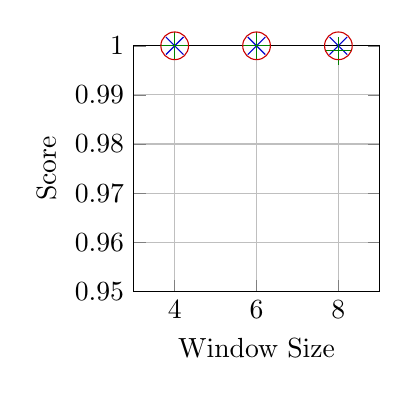
\begin{tikzpicture}
            \begin{axis}[
                xlabel={Window Size},
                ylabel={Score},
                xmin=3, xmax=9,
                ymin=0.95, ymax=1,
                xtick={4,6,8},
                ytick={0.95,0.96,0.97,0.98,0.99,1},
                width=4.7cm,
                height=4.7cm,
                grid=both,
                scatter/classes={
    step1={mark=x, mark size=4.5pt, draw=blue!80!black},
    step2={mark=+, mark size=5pt, draw=green!50!black},
    step3={mark=o, mark size=5pt, fill=red!50, draw=red!80!black}
},
                legend style={draw=none},
            ]
            \addplot[scatter, only marks, scatter src=explicit symbolic]
            coordinates {
                (4,1) [step1] 
                (6,1) [step1]
                (8,1) [step1]
                (4,1) [step2]
                (6,1) [step2]
                (8,0.999) [step2]
                (4,1) [step3]
                (6,1) [step3]
                (8,1) [step3]
            };
            \end{axis}
        \end{tikzpicture}
        }
        \vspace*{-0.43cm}
        \caption{\fontspec{Roboto} Precision}
    \end{subfigure}%
    \hspace{0.01\textwidth}%
    % Subfigure 2 - Recall
    \begin{subfigure}[t]{0.31\textwidth}
        \centering
        {\fontspec{Roboto}
        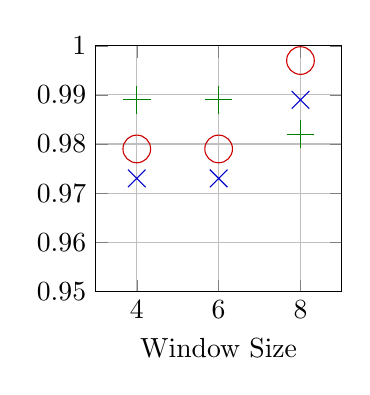
\begin{tikzpicture}
            \begin{axis}[
                xlabel={Window Size},
                xmin=3, xmax=9,
                ymin=0.95, ymax=1,
                xtick={4,6,8},
                ytick={0.95,0.96,0.97,0.98,0.99,1},
                width=4.7cm,
                height=4.7cm,
                grid=both,
                scatter/classes={
                      step1={mark=x, mark size=4.5pt, draw=blue!80!black},
    step2={mark=+, mark size=5pt, draw=green!50!black},
    step3={mark=o, mark size=5pt, fill=red!50, draw=red!80!black}
                },
                legend style={draw=none},
            ]
            \addplot[scatter, only marks, scatter src=explicit symbolic]
            coordinates {
                (4,0.973) [step1]
                (6,0.973) [step1]
                (8,0.989) [step1]
                (4,0.989) [step2]
                (6,0.989) [step2]
                (8,0.982) [step2]
                (4,0.979) [step3]
                (6,0.979) [step3]
                (8,0.997) [step3]
            };
            \end{axis}
        \end{tikzpicture}
        }
        \caption{\fontspec{Roboto} Recall}
    \end{subfigure}%
    \hspace{0.01\textwidth}%
    % Subfigure 3 - F1-Score
    \begin{subfigure}[t]{0.31\textwidth}
        \centering
        {\fontspec{Roboto}
        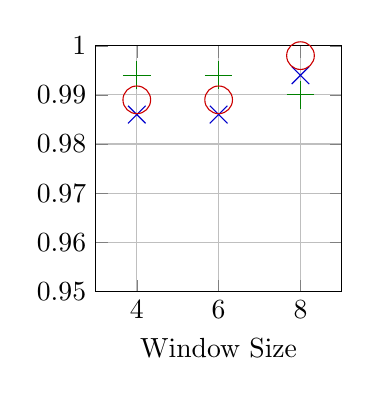
\begin{tikzpicture}
            \begin{axis}[
                xlabel={Window Size},
                xmin=3, xmax=9,
                ymin=0.95, ymax=1,
                xtick={4,6,8},
                ytick={0.95,0.96,0.97,0.98,0.99,1},
                width=4.7cm,
                height=4.7cm,
                grid=both,
                scatter/classes={
                      step1={mark=x, mark size=4.5pt, draw=blue!80!black},
                      step2={mark=+, mark size=5pt, draw=green!50!black},
                      step3={mark=o, mark size=5pt, fill=red!50, draw=red!80!black}},
                legend to name=sharedlegend,
                legend style={font = \fontspec{Roboto},draw=black, legend columns=3},
            ]
            \addplot[scatter, only marks, scatter src=explicit symbolic]
            coordinates {
                (4,0.986) [step1]
                (6,0.986) [step1]
                (8,0.994) [step1]
                (4,0.994) [step2]
                (6,0.994) [step2]
                (8,0.990) [step2]
                (4,0.989) [step3]
                (6,0.989) [step3]
                (8,0.998) [step3]
            };
            \legend{Step Size = 1, Step Size = 2, Step Size = 3}
            \end{axis}
        \end{tikzpicture}
        }
        \caption{\fontspec{Roboto} F1-score}
    \end{subfigure}

    \vspace{0.7cm}

    \caption{\revrev{}{Impact of window size and step size using SVM on the BGL dataset.}}
    \label{fig:svm_all_metrics}

    \vspace{0.5cm}
    \centering
  

\end{figure}

\subsubsection{Isolation Forest}
As seen in Figure \ref{fig:if_all_metrics} the window size has a big impact on all three evaluation metrics. Further, the step size has less impact, slightly affecting the results of each window size. For the three evaluated window sizes, precision, recall and F1-score exhibits similar trends. Notably, a window size of 6 hours consistently shows the weakest results, while a window size of 8 hours shows the highest results across all three metrics. The results consistently show that a window size of 4 and 8 hours performs best when paired with a step size of 3 hours, while window size of 6 hours performs best when paired with a step size of 1 hour. 

\begin{figure}[t]
    \centering
    % Shared legend at the very top, centered:
    \makebox[\textwidth]{\ref{sharedlegend}}
    \vspace{0.5cm} % Space between legend and subfigures
    % Subfigure 1 - Precision
    \begin{subfigure}[t]{0.31\textwidth}
        \centering
        {\fontspec{Roboto}
        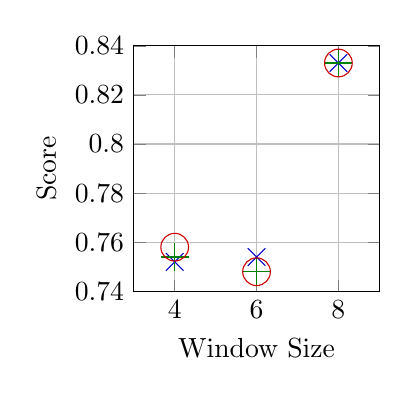
\begin{tikzpicture}
            \begin{axis}[
                xlabel={Window Size},
                ylabel={Score},
                xmin=3, xmax=9,
                ymin=0.74, ymax=0.84,
                xtick={4,6,8},
                ytick={0.74,0.76,0.78,0.80,0.82,0.84},
                width=4.7cm,
                height=4.7cm,
                grid=both,
                scatter/classes={
    step1={mark=x, mark size=4.5pt, draw=blue!80!black},
    step2={mark=+, mark size=5pt, draw=green!50!black},
    step3={mark=o, mark size=5pt, fill=red!50, draw=red!80!black}
},
                legend style={draw=none},
            ]
            \addplot[scatter, only marks, scatter src=explicit symbolic]
            coordinates {
                (4,0.752) [step1]
                (6,0.754) [step1]
                (8,0.833) [step1]
                (4,0.754) [step2]
                (6,0.748) [step2]
                (8,0.833) [step2]
                (4,0.758) [step3]
                (6,0.748) [step3]
                (8,0.833) [step3]
            };
            \end{axis}
        \end{tikzpicture}
        }
        \vspace*{-0.43cm}
        \caption{\fontspec{Roboto} Precision}
    \end{subfigure}%
    \hspace{0.01\textwidth}%
    % Subfigure 2 - Recall
    \begin{subfigure}[t]{0.31\textwidth}
        \centering
        {\fontspec{Roboto}
        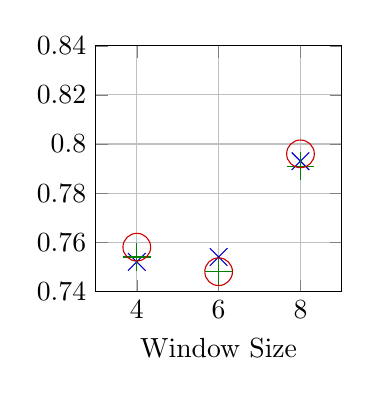
\begin{tikzpicture}
            \begin{axis}[
                xlabel={Window Size},
                xmin=3, xmax=9,
                ymin=0.74, ymax=0.84,
                xtick={4,6,8},
                ytick={0.74,0.76,0.78,0.80,0.82,0.84},
                width=4.7cm,
                height=4.7cm,
                grid=both,
                scatter/classes={
                      step1={mark=x, mark size=4.5pt, draw=blue!80!black},
    step2={mark=+, mark size=5pt, draw=green!50!black},
    step3={mark=o, mark size=5pt, fill=red!50, draw=red!80!black}
                },
                legend style={draw=none},
            ]
            \addplot[scatter, only marks, scatter src=explicit symbolic]
            coordinates {
                (4,0.752) [step1]
                (6,0.754) [step1]
                (8,0.793) [step1]
                (4,0.754) [step2]
                (6,0.748) [step2]
                (8,0.791) [step2]
                (4,0.758) [step3]
                (6,0.748) [step3]
                (8,0.796) [step3]
            };
            \end{axis}
        \end{tikzpicture}
        }
        \caption{\fontspec{Roboto} Recall}
    \end{subfigure}%
    \hspace{0.01\textwidth}%
    % Subfigure 3 - F1-Score
    \begin{subfigure}[t]{0.31\textwidth}
        \centering
        {\fontspec{Roboto}
        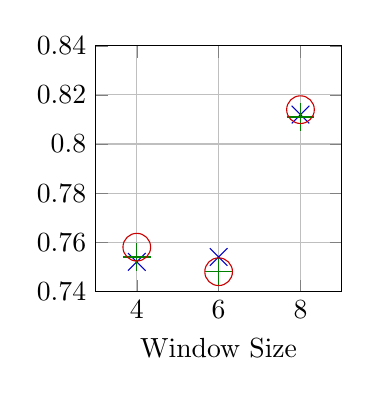
\begin{tikzpicture}
            \begin{axis}[
                xlabel={Window Size},
                xmin=3, xmax=9,
                ymin=0.74, ymax=0.84,
                xtick={4,6,8},
                ytick={0.74,0.76,0.78,0.80,0.82,0.84},
                width=4.7cm,
                height=4.7cm,
                grid=both,
                scatter/classes={
                      step1={mark=x, mark size=4.5pt, draw=blue!80!black},
                      step2={mark=+, mark size=5pt, draw=green!50!black},
                      step3={mark=o, mark size=5pt, fill=red!50, draw=red!80!black}},
                legend to name=sharedlegend,
                legend style={font = \fontspec{Roboto},draw=black, legend columns=3},
            ]
            \addplot[scatter, only marks, scatter src=explicit symbolic]
            coordinates {
                (4,0.752) [step1]
                (6,0.754) [step1]
                (8,0.812) [step1]
                (4,0.754) [step2]
                (6,0.748) [step2]
                (8,0.811) [step2]
                (4,0.758) [step3]
                (6,0.748) [step3]
                (8,0.814) [step3]
            };
            \legend{Step Size = 1, Step Size = 2, Step Size = 3}
            \end{axis}
        \end{tikzpicture}
        }
        \caption{\fontspec{Roboto} F1-score}
    \end{subfigure}

    \vspace{0.7cm}

    \caption{Impact of window size and step size using Isolation Forest on the BGL dataset.}
    \label{fig:if_all_metrics}

    \vspace{0.5cm}
    \centering
  

\end{figure}



\subsubsection{PCA}
The results for PCA are presented in Figure \ref{fig:pca_all_metrics}, where the precision is shown to be significantly higher when using an 8 hours window size. The recall results also show the best results when using an 8 hour window size, however the 4 hour window size exhibits the weakest recall, closely aligned to the results of the 6 hour window size. The F1-score is also the highest for the 8 hour window size, while the 4 and 6 hour window size show similar results, and the 2 hour step size gives the best results for all 3 window sizes. Once again, the step size has a minimal affect on the results for the three metrics, and the window size of 8 consistently outperformed the other configurations across all three metrics. 



\begin{figure}[t]
    \centering
    % Shared legend at the very top, centered:
    \makebox[\textwidth]{\ref{sharedlegend}}
    \vspace{0.5cm} % Space between legend and subfigures
    % Subfigure 1 - Precision
    \begin{subfigure}[t]{0.31\textwidth}
        \centering
        {\fontspec{Roboto}
        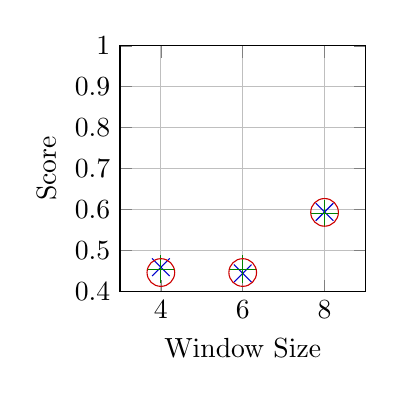
\begin{tikzpicture}
            \begin{axis}[
                xlabel={Window Size},
                ylabel={Score},
                xmin=3, xmax=9,
                ymin=0.4, ymax=1,
                xtick={4,6,8},
                ytick={0.4, 0.5, 0.6, 0.7, 0.8, 0.9, 1.0},
                width=4.7cm,
                height=4.7cm,
                grid=both,
                scatter/classes={
    step1={mark=x, mark size=4.5pt, draw=blue!80!black},
    step2={mark=+, mark size=5pt, draw=green!50!black},
    step3={mark=o, mark size=5pt, fill=red!50, draw=red!80!black}
},
                legend style={draw=none},
            ]
            \addplot[scatter, only marks, scatter src=explicit symbolic]
            coordinates {
               (4,0.459) [step1]
            (6,0.444) [step1]
            (8,0.594) [step1]
            (4,0.454) [step2]
            (6,0.454) [step2]
            (8,0.590) [step2]
            (4,0.446) [step3]
            (6,0.446) [step3]
            (8,0.593) [step3]
            };
            \end{axis}
        \end{tikzpicture}
        }
        \vspace*{-0.43cm}
        \caption{\fontspec{Roboto} Precision}
        \label{precisionPCABGL}
    \end{subfigure}%
    \hspace{0.01\textwidth}%
    % Subfigure 2 - Recall
    \begin{subfigure}[t]{0.31\textwidth}
        \centering
        {\fontspec{Roboto}
        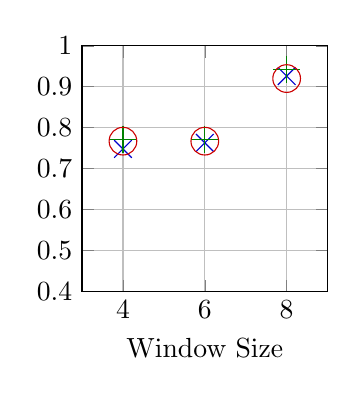
\begin{tikzpicture}
            \begin{axis}[
                xlabel={Window Size},
                xmin=3, xmax=9,
               ymin=0.4, ymax=1,
                xtick={4,6,8},
                ytick={0.4, 0.5, 0.6, 0.7, 0.8, 0.9,1.0},
                width=4.7cm,
                height=4.7cm,
                grid=both,
                scatter/classes={
                      step1={mark=x, mark size=4.5pt, draw=blue!80!black},
    step2={mark=+, mark size=5pt, draw=green!50!black},
    step3={mark=o, mark size=5pt, fill=red!50, draw=red!80!black}
                },
                legend style={draw=none},
            ]
            \addplot[scatter, only marks, scatter src=explicit symbolic]
            coordinates {
                (4,0.748) [step1]
            (6,0.763) [step1]
            (8,0.926) [step1]
            (4,0.771) [step2]
            (6,0.771) [step2]
            (8,0.942) [step2]
            (4,0.767) [step3]
            (6,0.767) [step3]
            (8,0.920) [step3]
            };
            \end{axis}
        \end{tikzpicture}
        }
        \caption{\fontspec{Roboto} Recall}
        \label{recallPCABGL}
    \end{subfigure}%
    \hspace{0.01\textwidth}%
    % Subfigure 3 - F1-Score
    \begin{subfigure}[t]{0.31\textwidth}
        \centering
        {\fontspec{Roboto}
        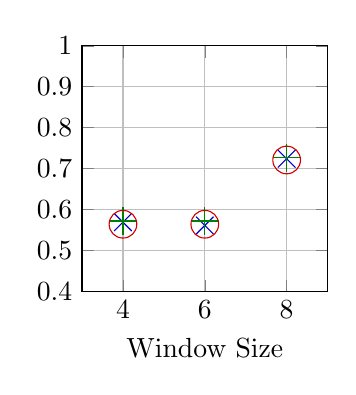
\begin{tikzpicture}
            \begin{axis}[
                xlabel={Window Size},
                xmin=3, xmax=9,
                ymin=0.4, ymax=1,
                xtick={4,6,8},
                ytick={0.4, 0.5, 0.6, 0.7, 0.8, 0.9,1.0},
                width=4.7cm,
                height=4.7cm,
                grid=both,
                scatter/classes={
                      step1={mark=x, mark size=4.5pt, draw=blue!80!black},
                      step2={mark=+, mark size=5pt, draw=green!50!black},
                      step3={mark=o, mark size=5pt, fill=red!50, draw=red!80!black}},
                legend to name=sharedlegend,
                legend style={font= \fontspec{Roboto},draw=black, legend columns=3},
            ]
            \addplot[scatter, only marks, scatter src=explicit symbolic]
            coordinates {
                (4,0.569) [step1]
            (6,0.561) [step1]
            (8,0.724) [step1]
            (4,0.572) [step2]
            (6,0.572) [step2]
            (8,0.726) [step2]
            (4,0.564) [step3]
            (6,0.564) [step3]
            (8,0.721) [step3]
            };
            \legend{Step Size = 1, Step Size = 2, Step Size = 3}
            \end{axis}
        \end{tikzpicture}
        
        }
        \caption{\fontspec{Roboto} F1-score}
    \end{subfigure}

    \vspace{0.7cm}

    \caption{Impact of window size and step size using PCA on the BGL dataset.}
    \label{fig:pca_all_metrics}
    \vspace{0.5cm}
    \centering
  

\end{figure}
\subsubsection{LogClustering}
The results for when LogClustering is applied on the BGL dataset are presented in Figure \ref{fig:logclustering_all_metrics}. Once again, it is evident that the 8-hour window size produces the best results. However, the step size has a more significant impact on the outcomes than previously, showing more noticeable variations in performance. Step size of 3 hours performs best when studying F1-score and recall, but a 2 hours step size provides the best results for precision. 


\begin{figure}[t]
    \centering
    % Shared legend at the very top, centered:
    \makebox[\textwidth]{\ref{sharedlegend}}
    \vspace{0.5cm} % Space between legend and subfigures
    % Subfigure 1 - Precision
    \begin{subfigure}[t]{0.31\textwidth}
        \centering
        {\fontspec{Roboto}
        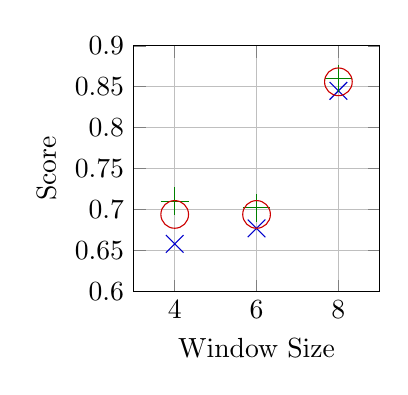
\begin{tikzpicture}
            \begin{axis}[
                xlabel={Window Size},
                ylabel={Score},
                xmin=3, xmax=9,
                ymin=0.6, ymax=0.9,
                xtick={4,6,8},
                ytick={0.60, 0.65, 0.70, 0.75, 0.80, 0.85, 0.90},
                width=4.7cm,
                height=4.7cm,
                grid=both,
                scatter/classes={
    step1={mark=x, mark size=4.5pt, draw=blue!80!black},
    step2={mark=+, mark size=5pt, draw=green!50!black},
    step3={mark=o, mark size=5pt, fill=red!50, draw=red!80!black}
},
                legend style={draw=none},
            ]
            \addplot[scatter, only marks, scatter src=explicit symbolic]
            coordinates {
                (4,0.658) [step1]
            (6,0.677) [step1]
            (8,0.845) [step1]
            (4,0.710) [step2]
            (6,0.702) [step2]
            (8,0.860) [step2]
            (4,0.694) [step3]
            (6,0.694) [step3]
            (8,0.856) [step3]
            };
            \end{axis}
        \end{tikzpicture}
        }
        \vspace*{-0.43cm}
        \caption{\fontspec{Roboto} Precision}
    \end{subfigure}%
    \hspace{0.01\textwidth}%
    % Subfigure 2 - Recall
    \begin{subfigure}[t]{0.31\textwidth}
        \centering
        {\fontspec{Roboto}
        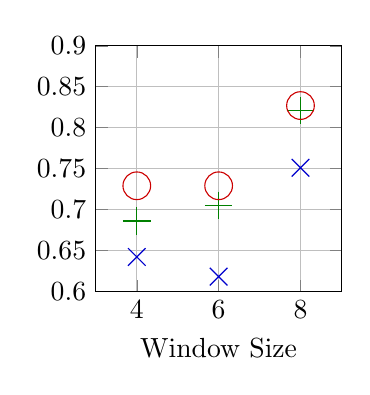
\begin{tikzpicture}
            \begin{axis}[
                xlabel={Window Size},
                xmin=3, xmax=9,
                ymin=0.6, ymax=0.9,
                xtick={4,6,8},
                ytick={0.60, 0.65, 0.70, 0.75, 0.80, 0.85, 0.90},
                width=4.7cm,
                height=4.7cm,
                grid=both,
                scatter/classes={
                      step1={mark=x, mark size=4.5pt, draw=blue!80!black},
    step2={mark=+, mark size=5pt, draw=green!50!black},
    step3={mark=o, mark size=5pt, fill=red!50, draw=red!80!black}
                },
                legend style={draw=none},
            ]
            \addplot[scatter, only marks, scatter src=explicit symbolic]
            coordinates {
                (4,0.642) [step1]
            (6,0.618) [step1]
            (8,0.751) [step1]
            (4,0.686) [step2]
            (6,0.705) [step2]
            (8,0.821) [step2]
            (4,0.729) [step3]
            (6,0.729) [step3]
            (8,0.827) [step3]
            };
            \end{axis}
        \end{tikzpicture}
        }
        \caption{\fontspec{Roboto} Recall}
    \end{subfigure}%
    \hspace{0.01\textwidth}%
    % Subfigure 3 - F1-Score
    \begin{subfigure}[t]{0.31\textwidth}
        \centering
        {\fontspec{Roboto}
        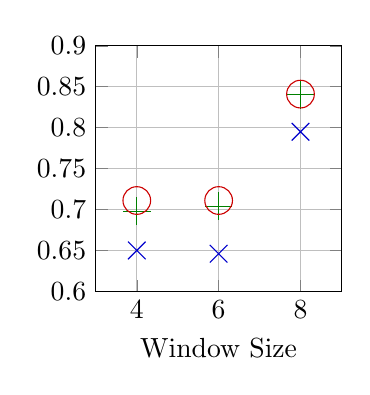
\begin{tikzpicture}
            \begin{axis}[
                xlabel={Window Size},
                xmin=3, xmax=9,
                ymin=0.6, ymax=0.9,
                xtick={4,6,8},
                ytick={0.60, 0.65, 0.70, 0.75, 0.80, 0.85, 0.90},
                width=4.7cm,
                height=4.7cm,
                grid=both,
                scatter/classes={
                      step1={mark=x, mark size=4.5pt, draw=blue!80!black},
                      step2={mark=+, mark size=5pt, draw=green!50!black},
                      step3={mark=o, mark size=5pt, fill=red!50, draw=red!80!black}},
                legend to name=sharedlegend,
                legend style={font=\fontspec{Roboto},draw=black, legend columns=3},
            ]
            \addplot[scatter, only marks, scatter src=explicit symbolic]
            coordinates {
                (4,0.650) [step1]
            (6,0.646) [step1]
            (8,0.795) [step1]
            (4,0.698) [step2]
            (6,0.704) [step2]
            (8,0.840) [step2]
            (4,0.711) [step3]
            (6,0.711) [step3]
            (8,0.841) [step3]
            };
            \legend{Step Size = 1, Step Size = 2, Step Size = 3}
            \end{axis}
        \end{tikzpicture}
        }
        \caption{\fontspec{Roboto} F1-score}
    \end{subfigure}

    \vspace{0.7cm}

    \caption{Impact of window size and step size using LogClustering on the BGL dataset.}
    \label{fig:logclustering_all_metrics}

    \vspace{0.5cm}
    \centering
  

\end{figure}





\subsubsection{Overall results for BGL}
Based on the tested window and step sizes, we selected the one with the best F1-score to represent the specific algorithm. The results of all algorithms when applied to the BGL datasets are shown in Figure \ref{fig:bgl-results}. \revrev{}{The benchmark algorithm SVM obtains the F1-score of 99.8\%. Studying the unsupervised methods,} LogClustering provides the best \revrev{F1 score}{F1-score}, demonstrates exceptional consistency across all three metrics. Isolation Forest also shows a stable result, with performance just below LogClustering. PCA provides the highest recall, but fairly weak results when studying the F1-score and precision. Studying the online methods results, One-Class SVM performs slightly better than HST on the BGL dataset, with a high recall. The BGL dataset contains significantly more unique log events compared to HDFS, resulting in a greater number of event combinations and a wider variety of anomalies. One-Class SVM can handle this better because of its use of continuous feature space, making it better at detecting hidden anomalies.

\begin{figure}[t]
    \centering
    {\fontspec{Roboto}
    \begin{tikzpicture}
        \begin{axis}[
            ybar,
            bar width=8pt,
            x=2.1cm,
            width=14cm,
            height=8cm,
            enlarge x limits=0.12,
            ylabel={Score},
            symbolic x coords={SVM, Isolation Forest, PCA, LogClustering, Half-Space Trees, One-Class SVM},
            xtick=data,
            xticklabel style={rotate=20, anchor=east},
            legend style={at={(0.97,0.97)}, anchor=north east, \fontspec{Roboto}},
            legend cell align=left,
            ymin=0, ymax=1.1,
            nodes near coords,
            nodes near coords align={vertical},
            every node near coord/.append style={font=\small},
            ylabel near ticks,
            axis x line*=bottom,
            axis y line*=left
        ]
        % Precision
        \addplot+[style={fill=blue!60}, bar shift=-17pt] coordinates {
            (SVM, 1)
            (Isolation Forest, 0.833) %window=8, step=3
            (PCA, 0.590) %window=8, step=2
            (LogClustering, 0.856) %window=8, step=3
            (Half-Space Trees, 0.143)
            (One-Class SVM, 0.1693)
        };
        % Recall
        \addplot+[style={fill=orange!70}, bar shift=0pt] coordinates {
            (SVM, 0.997)
            (Isolation Forest, 0.796) %window=8, step=3
            (PCA, 0.942) %window=8, step=2
            (LogClustering, 0.827) %window=8, step=3
            (Half-Space Trees, 0.358)
            (One-Class SVM, 0.5799)
        };
        % F1-score
        \addplot+[style={fill=green!60}, bar shift=17pt] coordinates {
        (SVM, 0.998)
            (Isolation Forest, 0.814) %window=8, step=3
            (PCA, 0.726) %window=8, step=2
            (LogClustering, 0.841) %window=8, step=3
            (Half-Space Trees, 0.205)
            (One-Class SVM, 0.2621)
        };
        \legend{Precision, Recall, F1-score}
        \end{axis}
    \end{tikzpicture}
    }
    \caption[Comparison of anomaly detection techniques on BGL dataset]{Comparison of anomaly detection techniques on BGL dataset \revrev{}{(results rounded to two decimal places)}.}
    \label{fig:bgl-results}
\end{figure}

\subsection{Offline vs Online}
This section presents the results for both offline and online algorithms when applied on the two datasets. In Figure \ref{fig:offline-vs-online-combined} the performance of the algorithms is averaged within each group by calculating the mean value \revrev{}{of the unsupervised algorithms (SVM excluded)}.


\begin{figure}[t]
    \centering
    {\fontspec{Roboto}
    % Shared legend
    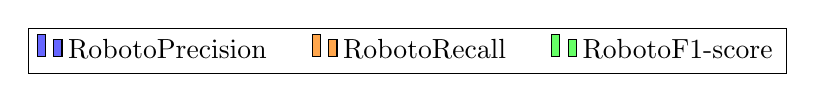
\begin{tikzpicture}
        \begin{axis}[
            hide axis,
            xmin=0, xmax=1,
            ymin=0, ymax=1,
            legend columns=3,
            legend style={
                at={(0.5,1.05)},
                anchor=south,
                draw=black,
                font=\fontspec{Roboto},
                /tikz/every even column/.append style={column sep=0.5cm}
            },
        ]
        \addlegendimage{ybar, ybar legend, fill=blue!60}
        \addlegendimage{ybar, ybar legend, fill=orange!70}
        \addlegendimage{ybar, ybar legend, fill=green!60}
        \addlegendentry{Precision}
        \addlegendentry{Recall}
        \addlegendentry{F1-score}
        \end{axis}
    \end{tikzpicture}

    % Subfigures
    \begin{subfigure}[t]{0.49\textwidth}
        \centering
       
        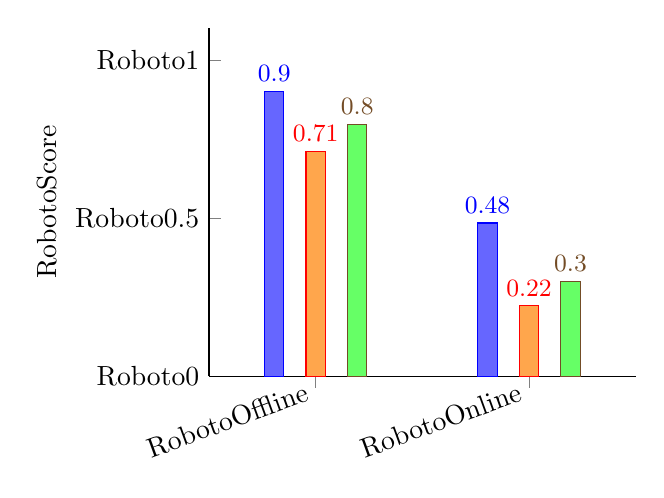
\begin{tikzpicture}
            \begin{axis}[
                font=\fontspec{Roboto},
                ybar,
                bar width=7pt,
                width=7cm,
                height=6cm,
                enlarge x limits=0.50,
                ylabel={Score},
                symbolic x coords={Offline, Online},
                xtick=data,
                xticklabel style={rotate=20, anchor=east},
                ymin=0, ymax=1.1,
                nodes near coords,
                nodes near coords align={vertical},
                every node near coord/.append style={font=\small},
                ylabel near ticks,
                axis x line*=bottom,
                axis y line*=left
            ]
            \addplot+[style={fill=blue!60}, bar shift=-15pt] coordinates {
                (Offline, 0.901)  
                (Online, 0.484) 
            };
            \addplot+[style={fill=orange!70}, bar shift=0pt] coordinates {
                (Offline, 0.711) 
                (Online, 0.222) 
            };
            \addplot+[style={fill=green!60}, bar shift=15pt] coordinates {
                (Offline, 0.795)
                (Online, 0.30)
            };
            \end{axis}
        \end{tikzpicture}
        \caption{\fontspec{Roboto} HDFS}
        \label{fig:HDFS-offline-vs-online-results}
    \end{subfigure}
    \hfill
    \begin{subfigure}[t]{0.49\textwidth}
       
        \centering
        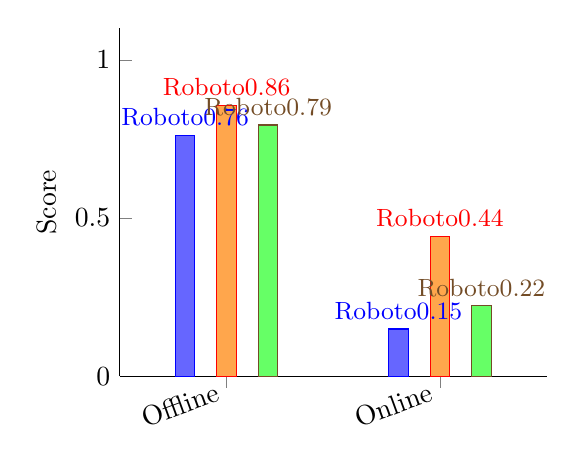
\begin{tikzpicture}
            \begin{axis}[
                ybar,
                bar width=7pt,
                width=7cm,
                height=6cm,
                enlarge x limits=0.50,
                ylabel={Score},
                symbolic x coords={Offline, Online},
                xtick=data,
                xticklabel style={rotate=20, anchor=east},
                ymin=0, ymax=1.1,
                nodes near coords,
                nodes near coords align={vertical},
                every node near coord/.append style={font=\small\fontspec{Roboto}},
                ylabel near ticks,
                axis x line*=bottom,
                axis y line*=left
            ]
            \addplot+[style={fill=blue!60}, bar shift=-15pt] coordinates {
                (Offline, 0.760)  
                (Online, 0.149) 
            };
            \addplot+[style={fill=orange!70}, bar shift=0pt] coordinates {
                (Offline, 0.855) 
                (Online, 0.442) 
            };
            \addplot+[style={fill=green!60}, bar shift=15pt] coordinates {
                (Offline, 0.794)
                (Online, 0.222)
            };
            \end{axis}
        \end{tikzpicture}
        \caption{\fontspec{Roboto} BGL}
        \label{fig:BGL-offline-vs-online-results}
    \end{subfigure}
    \caption[Offline vs Online performance on HDFS and BGL datasets]{Offline vs Online performance on HDFS and BGL datasets \revrev{}{(results rounded to two decimal places)}.}
    \label{fig:offline-vs-online-combined}
    }
\end{figure}

\subsubsection{HDFS}
As shown in Figure \ref{fig:HDFS-offline-vs-online-results}, the offline algorithms Isolation Forest, PCA and LogClustering perform much better than the online techniques Half-Space Trees and One-Class SVM on average. The offline methods result in a mean of $80$\% in F1-score, whereas the online algorithms only provide a mean of $30$\%. Notably, online methods produce significantly higher precision compared to recall. Offline techniques, on the other hand, maintain a more balanced relationship between precision and recall, despite a difference of $19$ percentage points. Offline methods are likely more stable due to the fact that they hold full access to the datasets during training. This enables them to capture underlying distribution, and model both normal and anomalous behavior better. The online methods instead operate incrementally with limited context, making them more conservative while also having more trouble to detect diverse anomaly patterns. This often leads to a lower recall, causing less stability for the online methods. 


\subsubsection{BGL}
For the BGL dataset, offline methods significantly outperform online techniques. As shown in Figure \ref{fig:BGL-offline-vs-online-results}, offline algorithms achieve an average F1-score of $79$\%, whereas online algorithms record a substantially lower F1-score of just $22$\%. In particular, online methods produce significantly higher recall compared to precision. Offline techniques, on the other hand, achieve a more balanced relationship between recall and precision.


\section{Summary of results}
The experimental results show that LogClustering performs the best on both datasets. When the algorithms are applied to the HDFS dataset, all algorithms show precision as its strongest metric. This does not go for the BGL dataset however, where the values are either close to each other or recall shows the highest value. Additionally, offline anomaly detectors outperform online anomaly detectors, delivering just above twice the performance across all three evaluation metrics. Among the online methods, Half-Space Trees achieved the best performance on the HDFS dataset, while One-Class SVM recorded the best results on the BGL dataset.

%%%%%%%%%%%%%%%%%%%%%%%%%%%%%%%%%%%%%%%%%%%%%%%%%%%%%%%%%%%%%%%%%%%%%%
%%% lorem.tex ends here

%%% Local Variables: 
%%% mode: latex
%%% TeX-master: "demothesis"
%%% End: 

%%% lorem.tex --- 
%% 
%% Filename: lorem.tex
%% Description: 
%% Author: Ola Leifler
%% Maintainer: 
%% Created: Wed Nov 10 09:59:23 2010 (CET)
%% Version: $Id$
%% Version: 
%% Last-Updated: Wed Nov 10 09:59:47 2010 (CET)
%%           By: Ola Leifler
%%     Update #: 2
%% URL: 
%% Keywords: 
%% Compatibility: 
%% 
%%%%%%%%%%%%%%%%%%%%%%%%%%%%%%%%%%%%%%%%%%%%%%%%%%%%%%%%%%%%%%%%%%%%%%
%% 
%%% Commentary: 
%% 
%% 
%% 
%%%%%%%%%%%%%%%%%%%%%%%%%%%%%%%%%%%%%%%%%%%%%%%%%%%%%%%%%%%%%%%%%%%%%%
%% 
%%% Change log:
%% 
%% 
%% RCS $Log$
%%%%%%%%%%%%%%%%%%%%%%%%%%%%%%%%%%%%%%%%%%%%%%%%%%%%%%%%%%%%%%%%%%%%%%
%% 
%%% Code:

\chapter{Discussion}
\label{cha:discussion}


\section{Results}
\label{sec:discussion-results}
In this section, we discuss the results from when applying the anomaly detection techniques on the different datasets and make comparisons between different algorithms.

\subsection{LogClustering}
The results clearly show that LogClustering performs the best on both datasets. This is likely because LogClustering uses a knowledge base with stored sequences from each cluster, which it can compare new sequences to. Looking at sequences works particularly well for system log files, since anomalies are often characterized by a typical event pattern. Additionally, since LogClustering is the only anomaly detection method which requires normal training data, it makes it easier to separate the normal clusters from anomalous in the evaluating phase. Although it might seem unfair to let LogClustering train on normal data while the other techniques don't, this report aims to find the best technique for online and offline scenarios. A offline real-world scenario would include knowing what normal logdata looks like, therefore it's not unreasonable to compare LogClustering to the others, giving each method what it needs to reach it's full potential. Further analyzing the results of LogClustering we see that it performs slightly better on the HDFS dataset than the BGL dataset. While this could be due to the different feature extraction techniques, it's not likely the main reason since the overall results show that offline techniques generate an F1-score of $80$\% on the HDFS data and $79$\% on the BGL data. These results are more likely due to the different dimensions, where $49$ unique event IDs were generated from the HDFS dataset, compared to BGL's $320$. More event IDs creates a high-dimensional and sparse event count matrix, making it difficult for the clustering to separate normal instances from anomalous, generating more false positives \cite{Shilin2017experiencereport}. This claim is further supported by the lower precision for when LogClustering is applied to the BGL data, compared to the $100$\% precision on the HDFS data.

\revrev{}{Lastly, when comparing LogClustering to the benchmark (SVM) on HDFS, we see that the F1-score is approximately 8 percentage points lower, but the precision performs better. However, this only indicates that LogClustering is precise, and that all data points classified as anomalies are indeed true anomalies. The lower recall of 81\% however indicates that it fails to capture all actual anomalies. The difference on BGL is larger, with a F1-score difference of approximately 16 percentage points, indicating that the higher complexity in BGL is harder to handle without labels.}
 
\subsection{PCA}
The PCA algorithm gave a poor precision result, only $59$\%, on the BGL dataset and made it the worst method among the three offline techniques. This may be because PCA identifies unusual data by measuring how much a point deviates from normal patterns and a single threshold might not be enough to capture a lot anomalies without many false positives \cite{Shilin2017experiencereport}. On the other hand, PCA produces a notably higher precision, $95$\%, for the HDFS dataset. The big difference between the algorithms performance on the datasets could be because the HDFS dataset was feature extracted using a session window method, whereas the BGL dataset used a sliding window approach. This introduces more variability and noise in the anomaly data, as further discussed in Section \ref{sec:discussion-method}. Our results also showed that it was easier to find anomalies in the BGL data (higher recall), this could also be due to the different feature extraction approaches. Overall the PCA algorithm provided higher precision on the HDFS dataset, resulting in a higher F1-score and therefore performing better on the HDFS data. \revrev{}{The PCA algorithm achieved an F1-score approximately 27 percentage points lower on the BGL data than the SVM benchmark technique. This significant difference indicates that PCA is far from perfect for this type of data. On the HDFS data, PCA was slightly closer to the SVM algorithm, now with a difference of approximately 15 percentage points in F1-score.}

\subsection{Isolation Forest}
Isolation Forest is the only offline algorithm that presents better results on the BGL data compared with the HDFS data. \revrev{}{Its performance on the HDFS dataset is significantly worse than the benchmark, with an \revrev{F1 score}{F1-score} that is 29 percentage points lower, compared to 19 percentage points lower on the BGL dataset.} The biggest difference seen when evaluating the results on the two datasets is that the recall is notably higher for the BGL dataset. Also, the precision is higher, but the difference is not as big. This indicates that even though BGL is feature extracted by a sliding window approach, the tree algorithm, Isolation Forest, manages to increase the precision slightly, which is a bit contradictory to what’s said in Section \ref{sec:discussion-method}. This leads to the conclusion that Isolation Forest handles noise that comes from the sliding window approach better than the other offline algorithms. It could also be that tree algorithms like Isolation Forest work better for sliding window approaches in an offline environment, but more research would need to be done on other tree algorithms to reach that conclusion.


\subsection{The online methods}
When comparing the online methods, the results lie fairly close to each other. Half-Space Trees (HST) performed best on the HDFS data, while One-Class SVM performed better on the BGL dataset. HDFS consists of fewer anomalous data points, and as mentioned in Section \ref{HST}, HST is particularly effective for datasets with few anomalous data points. This is also proven in our experimental results, where HST delivers an F1-score of $33$\% on HDFS compared to $21$\% on the BGL data. 

Furthermore, since BGL contains significantly more unique events than the HDFS dataset, this creates more unique combinations of events and anomalies. One-Class SVM can therefore achieve a better result on the BGL dataset than HST, since it has the ability to learn a compact decision boundary around the normal data in its feature space. \revrev{}{Also, it's kernel function helps dealing with complex and non-linear patterns, transforming input data into a higher dimensional space where linnear separation is possible.} This makes \revrev{a}{} One-Class SVM generalize better in scenarios with high variability, allowing it to detect anomalies that do not follow consistent patterns. In contrast, fewer unique events in the HDFS dataset makes HST more compatible, since the lower complexity results in a narrower range of event patterns and anomaly types. This suits HST and its way of isolating anomalies, which works well when anomalies clearly deviate from the normal data.

Although both have precision as its best performing metric in HDFS, and recall as its best performing metric on BGL, this is in line with what is suggested in Section \ref{sec:discussion-method}.

\subsection{Comparing online to offline anomaly detection}
The experimental results demonstrate that the offline approaches decisively outperform the online methods. These results comes with no surprises however, as the offline methods are training on the entire datasets, while the online methods are only trained on 80\% giving the offline methods more data to learn from. This also gives them the opportunity to score based on historical and future knowledge, while the online methods can only score based on historical knowledge. Additionally, the feature extraction will perform differently in the two scenarios. In the offline setting, complete feature vectors will be constructed throughout the entire dataset before any scoring takes place. Giving the anomaly detection model access to richer and more context-aware features. The online scenario on the other hand, must process logs incrementally, scoring row by row as the new data arrives. Therefore the feature vectors are updated dynamically, sometimes with incomplete contextual information. This fundamental limitation contributes to the performance gap between offline and online settings. 

\section{Method}
\label{sec:discussion-method}
Our feature extraction methods differed between the two datasets. The HDFS dataset included block IDs for each log entry and that allowed for a session window approach to be used. Since each log row was associated with a specific block ID, we could label entire blocks as either anomalous or normal. In contrast, the BGL dataset didn't have such identifiers, hindering the use of a session-based approach. Instead, we applied a sliding window method, where windows were classified as anomalous if they contained one or more anomalous log entries.

This difference in feature extraction had a considerable impact on performance. The session window approach led to higher precision, as anomalies were easier to identify\revrev{ .}{, likely because the vectors were grouped by \textit{block\_id}, which were already labeled as either anomalous or normal. This decreases the chances of false positives.} On the other hand, the sliding window method resulted in higher recall, since several anomalies and normals could be in the same window. This caused some windows to be labeled as anomalous even if they included events that were actually normal. \revrev{}{This leads to a higher recall since more actual anomalies are captured, but lower precision due to an increased number of false positives}. 

For the sliding window approach applied to the offline algorithms on the BGL dataset, we found that the step size had minimal impact on the results. The window size, on the other hand, had a significant effect on the results. This is likely because the step size only controls how frequently a new window is generated, without changing much of the actual content in each window. However, changes in window size affect what data is included within each window, which can be the determining factor in whether a window is classified as anomalous or normal.

Even though the largest window size (eight hours) consistently showed the best results for the offline algorithms, it also comes with some negative effects. A high window size means that we know that at least one anomaly exists within the window but we don't know exactly which log entry is anomalous or how many anomalies are present. As a result, manual inspection is required to find the anomalies, and a larger window leads to more log entries to examine. In summary, a larger window size improves the performance but increases the effort and time needed for analysis.

\subsection{Limitations}
Our results showed a notable performance gap between the online and offline algorithms. One key reason for this difference is that the online algorithms required longer runtime, which limited our ability to tune their parameters to the same extent as we did for the offline algorithms. For example, with Half-Space Trees the ideal would be to experiment with the number of trees and their height, but increasing these parameters made the algorithm unable to run within a reasonable time on our datasets and hardware. Likewise, One-Class SVM had a long runtime even with default settings, which made it difficult to work iteratively and explore parameter adjustments. Additionally, we were not able to adjust the window sizes for the online algorithms on the BGL dataset. The online techniques became very slow when modifying the window size, which prevented us from testing different window sizes. 

We provided the different algorithms with event IDs based on log templates. It means that the algorithms only had access to one type of parameter, the amount of times a specific event occurred. It could be beneficial to provide more parameters, such as size, timestamp and addresses, for better results and making it easier for the algorithm to detect anomalies. 

\section{The work in a wider context}
\label{sec:work-wider-context}
The collection and analysis of log data could raise some ethical questions due to different reasons. Firstly, using machine learning approaches for anomaly detection studies user behavior, and it should be made sure that the work follows laws and regulations such as GDPR, and the processing of data should ensure privacy for individuals \cite{Devineni2023datasecurityandintegrity}. Also, the suggested machine learning models almost always find some false positives. This can lead to falsely accusing a user for abnormal behavior, creating ethical concerns. Lastly, the data handled could be considered sensitive, and as Devineni et al.\cite{Devineni2023datasecurityandintegrity} claims, it is critical that data can be anonymized or receives secure encryption. However, fighting these challenges without affecting the results of the machine learning techniques is not self-evident.


%%%%%%%%%%%%%%%%%%%%%%%%%%%%%%%%%%%%%%%%%%%%%%%%%%%%%%%%%%%%%%%%%%%%%%
%%% lorem.tex ends here

%%% Local Variables: 
%%% mode: latex
%%% TeX-master: "demothesis"
%%% End: 


%%% lorem.tex --- 
%% 
%% Filename: lorem.tex
%% Description: 
%% Author: Ola Leifler
%% Maintainer: 
%% Created: Wed Nov 10 09:59:23 2010 (CET)
%% Version: $Id$
%% Version: 
%% Last-Updated: Wed Nov 10 09:59:47 2010 (CET)
%%           By: Ola Leifler
%%     Update #: 2
%% URL: 
%% Keywords: 
%% Compatibility: 
%% 
%%%%%%%%%%%%%%%%%%%%%%%%%%%%%%%%%%%%%%%%%%%%%%%%%%%%%%%%%%%%%%%%%%%%%%
%% 
%%% Commentary: 
%% 
%% 
%% 
%%%%%%%%%%%%%%%%%%%%%%%%%%%%%%%%%%%%%%%%%%%%%%%%%%%%%%%%%%%%%%%%%%%%%%
%% 
%%% Change log:
%% 
%% 
%% RCS $Log$
%%%%%%%%%%%%%%%%%%%%%%%%%%%%%%%%%%%%%%%%%%%%%%%%%%%%%%%%%%%%%%%%%%%%%%
%% 
%%% Code:

\chapter{Conclusion}
\label{cha:conclusion}

In this thesis, we have shown that LogClustering is the best performing offline algorithm based on all three evaluation metrics (precision, recall and F1) on the HDFS and BGL dataset. As LogClustering uses a knowledge base, with stored sequences from each cluster which it compares new sequences to, it is highly suitable for system log files analysis. Additionally, LogClustering is the only technique out of the three offline which trains on normal data, making it easier to separate anomalous data when arriving in the testing phase. Therefore, LogClustering performs better than Isolation Forest and PCA in an offline setting. 

This study compared two online anomaly detection techniques, Half-Space Trees and an online implementation of One-Class SVM, each implemented on two datasets, HDFS and BGL. In this case, the results do not indicate a best performing algorithm, as Half-Space Trees performed slightly better on the HDFS dataset, and One-Class SVM performed better on the BGL dataset. HST is however particularly effective when applied to datasets with few anomalous data points, which is proven since it performs better on HDFS which contains less anomalies than BGL. Further, One-Class SVM performs better on dataset with more complex, deviated anomalies than HST, due to it's feature space boundary. With this said, HST is the more suitable algorithm when the proportion of anomalies within the dataset is relatively low, and easy to isolate. While One-Class SVM is better suited on scenarios with a more complex, deviated, and higher percentage of anomalies.

The results for the offline and online anomaly detection techniques differed severely. Offline performed significantly better in regards to all three evaluation metrics. The average F1-score was $50$ percentage points higher for the offline methods on the HDFS data and $57$ percentage points higher on the BGL dataset. There are several reasons behind this, the biggest being that offline methods trained on the full dataset and online methods only trained on $80$\%. Also, since offline algorithms have access to the data the evaluation is performed on beforehand which has a huge impact. Lastly, a reason for the big result gap is that the online methods was much slower and our experimental setup couldn't handle tweaking the parameters of the algorithms as we did with the offline techniques.  

The conclusions made us achieve our aim of comparing various anomaly detection techniques in different non-encrypted log datasets. We found \revrev{what algorithm was the best}{which algorithm performed best
} on two different datasets and compared the two different use cases, offline and online, which also was a part of the aim for this study.

\section{Future work}
As this study investigates online and offline anomaly detection on log data, evaluating the three metrics precision, recall and F1-score, it leaves space for future work. The need \revrev{of}{for} online anomaly detection is huge, and there are more anomaly \revrev{detections}{detection} techniques to be investigated. Further, finding anomalies \revrev{are}{is} important, and the three metrics are fully relevant. However in an online setting additional factors as CPU usage and running time \revrev{comes of importance}{is of importance}. This thesis provides a good foundation to further investigate these metrics, with the potential to further strengthen security on log data. \revrev{}{Also, to better judge the potential of the online algorithms, future work should focus on tuning their parameters. As improved tuning may lead to more fair comparisons and reveal whether the current performance gap between offline and online models is due to limitations in the models or simply a lack of optimization.}
Because of a limited time scope, this thesis used one general method with one log parsing technique, two different feature extractors and five anomaly detection techniques applied on two different datasets. It would be interesting for future research to compare other factors than anomaly detection, such as general methods, log parsing and more feature extractors to see how preprocessing data affects the overall result. Additionally, studying more datasets, with different structures would help \revrev{}{in} finding the best solutions for different situations. 

%%%%%%%%%%%%%%%%%%%%%%%%%%%%%%%%%%%%%%%%%%%%%%%%%%%%%%%%%%%%%%%%%%%%%%
%%% lorem.tex ends here

%%% Local Variables: 
%%% mode: latex
%%% TeX-master: "demothesis"
%%% End: 

\printbibliography
\end{document}
